% Generated by scripts/fault_tree_figure.py.
\definecolor{ftT}{HTML}{E3EDFA}\definecolor{ftTb}{HTML}{2A78D6}
\definecolor{ftH}{HTML}{FDEBD9}\definecolor{ftHb}{HTML}{C26A14}
\definecolor{ftO}{HTML}{EFE6F6}\definecolor{ftOb}{HTML}{7C3AED}
\definecolor{ftE}{HTML}{E6F2E0}\definecolor{ftEb}{HTML}{3F7D2A}
\definecolor{ftG}{HTML}{1F2937}\definecolor{ftL}{HTML}{6B7280}
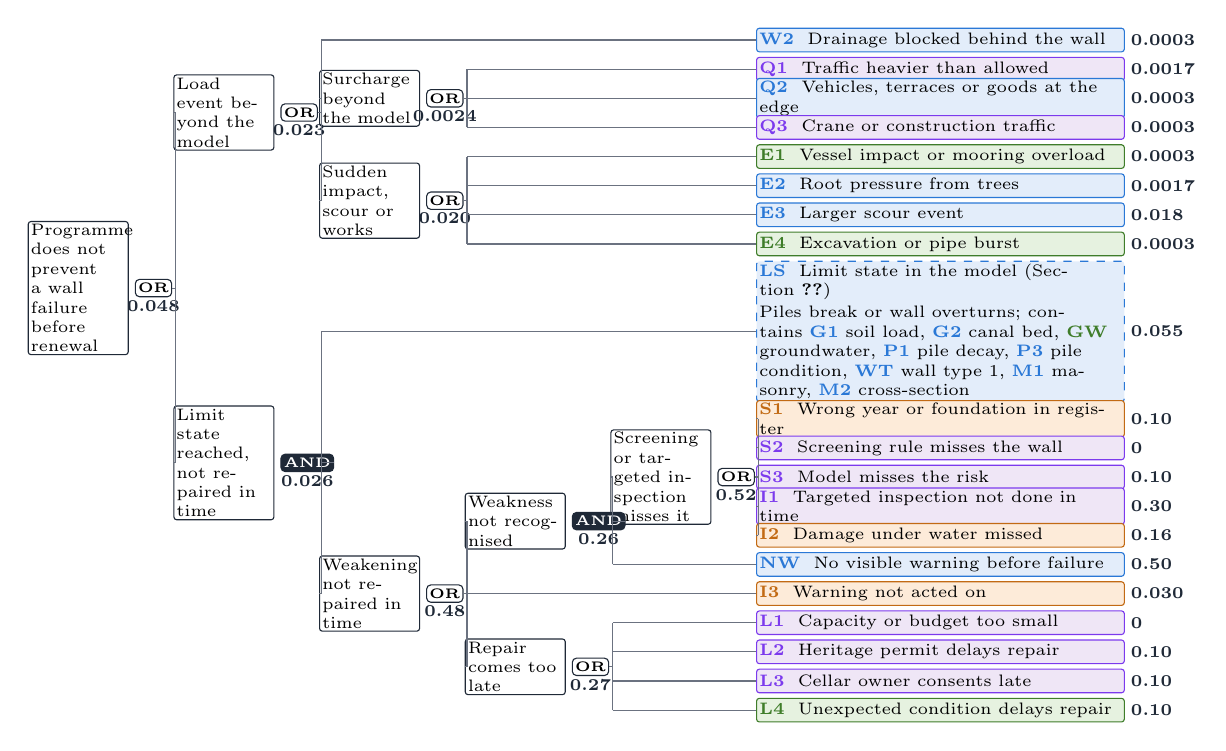
\begin{tikzpicture}[x=1cm,y=1cm,font=\fontsize{6.2}{7}\selectfont,every node/.style={inner sep=1pt}]
\tikzset{gate/.style={draw=ftG,fill=white,rounded corners=1.5pt,font=\fontsize{5}{5}\selectfont\bfseries,minimum width=0.42cm,minimum height=0.22cm},andgate/.style={gate,fill=ftG,text=white},ev/.style={draw=ftG,fill=white,rounded corners=1pt,align=left,text width=1.2cm,minimum height=0.3cm},line/.style={ftL,line width=0.4pt},pv/.style={font=\fontsize{5.6}{6}\selectfont\bfseries,text=ftG}}
\node[draw=ftTb,fill=ftT,rounded corners=1pt,anchor=west,minimum height=0.3cm,text width=4.6cm] at (9.25,0.00) {\textbf{\color{ftTb}W2}\ \ Drainage blocked behind the wall};
\node[pv,anchor=west] at (13.97,0.00) {0.0003};
\node[draw=ftOb,fill=ftO,rounded corners=1pt,anchor=west,minimum height=0.3cm,text width=4.6cm] at (9.25,-0.37) {\textbf{\color{ftOb}Q1}\ \ Traffic heavier than allowed};
\node[pv,anchor=west] at (13.97,-0.37) {0.0017};
\node[draw=ftTb,fill=ftT,rounded corners=1pt,anchor=west,minimum height=0.3cm,text width=4.6cm] at (9.25,-0.74) {\textbf{\color{ftTb}Q2}\ \ Vehicles, terraces or goods at the edge};
\node[pv,anchor=west] at (13.97,-0.74) {0.0003};
\node[draw=ftOb,fill=ftO,rounded corners=1pt,anchor=west,minimum height=0.3cm,text width=4.6cm] at (9.25,-1.11) {\textbf{\color{ftOb}Q3}\ \ Crane or construction traffic};
\node[pv,anchor=west] at (13.97,-1.11) {0.0003};
\node[ev,anchor=west] at (3.70,-0.74) {Surcharge beyond the model};
\node[gate,anchor=west] (g) at (5.06,-0.74) {OR};
\node[pv,anchor=north] at (g.south) {0.0024};
\draw[line] (g.east) -- (5.58,-0.74);
\draw[line] (5.58,-1.11) -- (5.58,-0.37);
\draw[line] (5.58,-0.37) -- (9.25,-0.37);
\draw[line] (5.58,-0.74) -- (9.25,-0.74);
\draw[line] (5.58,-1.11) -- (9.25,-1.11);
\node[draw=ftEb,fill=ftE,rounded corners=1pt,anchor=west,minimum height=0.3cm,text width=4.6cm] at (9.25,-1.48) {\textbf{\color{ftEb}E1}\ \ Vessel impact or mooring overload};
\node[pv,anchor=west] at (13.97,-1.48) {0.0003};
\node[draw=ftTb,fill=ftT,rounded corners=1pt,anchor=west,minimum height=0.3cm,text width=4.6cm] at (9.25,-1.85) {\textbf{\color{ftTb}E2}\ \ Root pressure from trees};
\node[pv,anchor=west] at (13.97,-1.85) {0.0017};
\node[draw=ftTb,fill=ftT,rounded corners=1pt,anchor=west,minimum height=0.3cm,text width=4.6cm] at (9.25,-2.22) {\textbf{\color{ftTb}E3}\ \ Larger scour event};
\node[pv,anchor=west] at (13.97,-2.22) {0.018};
\node[draw=ftEb,fill=ftE,rounded corners=1pt,anchor=west,minimum height=0.3cm,text width=4.6cm] at (9.25,-2.59) {\textbf{\color{ftEb}E4}\ \ Excavation or pipe burst};
\node[pv,anchor=west] at (13.97,-2.59) {0.0003};
\node[ev,anchor=west] at (3.70,-2.04) {Sudden impact, scour or works};
\node[gate,anchor=west] (g) at (5.06,-2.04) {OR};
\node[pv,anchor=north] at (g.south) {0.020};
\draw[line] (g.east) -- (5.58,-2.04);
\draw[line] (5.58,-2.59) -- (5.58,-1.48);
\draw[line] (5.58,-1.48) -- (9.25,-1.48);
\draw[line] (5.58,-1.85) -- (9.25,-1.85);
\draw[line] (5.58,-2.22) -- (9.25,-2.22);
\draw[line] (5.58,-2.59) -- (9.25,-2.59);
\node[ev,anchor=west] at (1.85,-0.92) {Load event beyond the model};
\node[gate,anchor=west] (g) at (3.21,-0.92) {OR};
\node[pv,anchor=north] at (g.south) {0.023};
\draw[line] (g.east) -- (3.73,-0.92);
\draw[line] (3.73,-2.04) -- (3.73,0.00);
\draw[line] (3.73,0.00) -- (9.25,0.00);
\draw[line] (3.73,-0.74) -- (3.70,-0.74);
\draw[line] (3.73,-2.04) -- (3.70,-2.04);
\node[draw=ftTb,fill=ftT,dashed,rounded corners=1pt,anchor=west,align=left,text width=4.6cm] at (9.25,-3.70) {\textbf{\color{ftTb}LS}\ \ Limit state in the model (Section~\ref{sec:prob})\\[1pt]{\fontsize{5.6}{6.6}\selectfont Piles break or wall overturns; contains \textbf{\color{ftTb}G1} soil load, \textbf{\color{ftTb}G2} canal bed, \textbf{\color{ftEb}GW} groundwater, \textbf{\color{ftTb}P1} pile decay, \textbf{\color{ftTb}P3} pile condition, \textbf{\color{ftTb}WT} wall type~1, \textbf{\color{ftTb}M1} masonry, \textbf{\color{ftTb}M2} cross-section}};
\node[pv,anchor=west] at (13.97,-3.70) {0.055};
\node[draw=ftHb,fill=ftH,rounded corners=1pt,anchor=west,minimum height=0.3cm,text width=4.6cm] at (9.25,-4.81) {\textbf{\color{ftHb}S1}\ \ Wrong year or foundation in register};
\node[pv,anchor=west] at (13.97,-4.81) {0.10};
\node[draw=ftOb,fill=ftO,rounded corners=1pt,anchor=west,minimum height=0.3cm,text width=4.6cm] at (9.25,-5.18) {\textbf{\color{ftOb}S2}\ \ Screening rule misses the wall};
\node[pv,anchor=west] at (13.97,-5.18) {0};
\node[draw=ftOb,fill=ftO,rounded corners=1pt,anchor=west,minimum height=0.3cm,text width=4.6cm] at (9.25,-5.55) {\textbf{\color{ftOb}S3}\ \ Model misses the risk};
\node[pv,anchor=west] at (13.97,-5.55) {0.10};
\node[draw=ftOb,fill=ftO,rounded corners=1pt,anchor=west,minimum height=0.3cm,text width=4.6cm] at (9.25,-5.92) {\textbf{\color{ftOb}I1}\ \ Targeted inspection not done in time};
\node[pv,anchor=west] at (13.97,-5.92) {0.30};
\node[draw=ftHb,fill=ftH,rounded corners=1pt,anchor=west,minimum height=0.3cm,text width=4.6cm] at (9.25,-6.29) {\textbf{\color{ftHb}I2}\ \ Damage under water missed};
\node[pv,anchor=west] at (13.97,-6.29) {0.16};
\node[ev,anchor=west] at (7.40,-5.55) {Screening or targeted inspection misses it};
\node[gate,anchor=west] (g) at (8.76,-5.55) {OR};
\node[pv,anchor=north] at (g.south) {0.52};
\draw[line] (g.east) -- (9.28,-5.55);
\draw[line] (9.28,-6.29) -- (9.28,-4.81);
\draw[line] (9.28,-4.81) -- (9.25,-4.81);
\draw[line] (9.28,-5.18) -- (9.25,-5.18);
\draw[line] (9.28,-5.55) -- (9.25,-5.55);
\draw[line] (9.28,-5.92) -- (9.25,-5.92);
\draw[line] (9.28,-6.29) -- (9.25,-6.29);
\node[draw=ftTb,fill=ftT,rounded corners=1pt,anchor=west,minimum height=0.3cm,text width=4.6cm] at (9.25,-6.66) {\textbf{\color{ftTb}NW}\ \ No visible warning before failure};
\node[pv,anchor=west] at (13.97,-6.66) {0.50};
\node[ev,anchor=west] at (5.55,-6.11) {Weakness not recognised};
\node[andgate,anchor=west] (g) at (6.91,-6.11) {AND};
\node[pv,anchor=north] at (g.south) {0.26};
\draw[line] (g.east) -- (7.43,-6.11);
\draw[line] (7.43,-6.66) -- (7.43,-5.55);
\draw[line] (7.43,-5.55) -- (7.40,-5.55);
\draw[line] (7.43,-6.66) -- (9.25,-6.66);
\node[draw=ftHb,fill=ftH,rounded corners=1pt,anchor=west,minimum height=0.3cm,text width=4.6cm] at (9.25,-7.03) {\textbf{\color{ftHb}I3}\ \ Warning not acted on};
\node[pv,anchor=west] at (13.97,-7.03) {0.030};
\node[draw=ftOb,fill=ftO,rounded corners=1pt,anchor=west,minimum height=0.3cm,text width=4.6cm] at (9.25,-7.40) {\textbf{\color{ftOb}L1}\ \ Capacity or budget too small};
\node[pv,anchor=west] at (13.97,-7.40) {0};
\node[draw=ftOb,fill=ftO,rounded corners=1pt,anchor=west,minimum height=0.3cm,text width=4.6cm] at (9.25,-7.77) {\textbf{\color{ftOb}L2}\ \ Heritage permit delays repair};
\node[pv,anchor=west] at (13.97,-7.77) {0.10};
\node[draw=ftOb,fill=ftO,rounded corners=1pt,anchor=west,minimum height=0.3cm,text width=4.6cm] at (9.25,-8.14) {\textbf{\color{ftOb}L3}\ \ Cellar owner consents late};
\node[pv,anchor=west] at (13.97,-8.14) {0.10};
\node[draw=ftEb,fill=ftE,rounded corners=1pt,anchor=west,minimum height=0.3cm,text width=4.6cm] at (9.25,-8.51) {\textbf{\color{ftEb}L4}\ \ Unexpected condition delays repair};
\node[pv,anchor=west] at (13.97,-8.51) {0.10};
\node[ev,anchor=west] at (5.55,-7.96) {Repair comes too late};
\node[gate,anchor=west] (g) at (6.91,-7.96) {OR};
\node[pv,anchor=north] at (g.south) {0.27};
\draw[line] (g.east) -- (7.43,-7.96);
\draw[line] (7.43,-8.51) -- (7.43,-7.40);
\draw[line] (7.43,-7.40) -- (9.25,-7.40);
\draw[line] (7.43,-7.77) -- (9.25,-7.77);
\draw[line] (7.43,-8.14) -- (9.25,-8.14);
\draw[line] (7.43,-8.51) -- (9.25,-8.51);
\node[ev,anchor=west] at (3.70,-7.03) {Weakening not repaired in time};
\node[gate,anchor=west] (g) at (5.06,-7.03) {OR};
\node[pv,anchor=north] at (g.south) {0.48};
\draw[line] (g.east) -- (5.58,-7.03);
\draw[line] (5.58,-7.96) -- (5.58,-6.11);
\draw[line] (5.58,-6.11) -- (5.55,-6.11);
\draw[line] (5.58,-7.03) -- (9.25,-7.03);
\draw[line] (5.58,-7.96) -- (5.55,-7.96);
\node[ev,anchor=west] at (1.85,-5.37) {Limit state reached, not repaired in time};
\node[andgate,anchor=west] (g) at (3.21,-5.37) {AND};
\node[pv,anchor=north] at (g.south) {0.026};
\draw[line] (g.east) -- (3.73,-5.37);
\draw[line] (3.73,-7.03) -- (3.73,-3.70);
\draw[line] (3.73,-3.70) -- (9.25,-3.70);
\draw[line] (3.73,-7.03) -- (3.70,-7.03);
\node[ev,anchor=west] at (0.00,-3.15) {Programme does not prevent a wall failure before renewal};
\node[gate,anchor=west] (g) at (1.36,-3.15) {OR};
\node[pv,anchor=north] at (g.south) {0.048};
\draw[line] (g.east) -- (1.88,-3.15);
\draw[line] (1.88,-5.37) -- (1.88,-0.92);
\draw[line] (1.88,-0.92) -- (1.85,-0.92);
\draw[line] (1.88,-5.37) -- (1.85,-5.37);
\end{tikzpicture}
